%%%%%%%%%%%%%%%%%%%%%%%%%%%%%%%%%%%%%%%%%%%%%%%%%%%%%%%%%%%%%%%%%%%%%%%%%%%%%%%
\documentclass[hyperref={pdfpagelabels=false},compress,table]{beamer} % 在Mac下无法编译
% \documentclass[compress,table]{beamer} % 在Mac下使用
% package for font
\usepackage{fontspec}
\defaultfontfeatures{Mapping=tex-text}  %%如果没有它,会有一些 tex 特殊字符无法正常使用,比如连字符。
\usepackage{xunicode,xltxtra}
\usepackage[BoldFont,SlantFont,CJKnumber,CJKchecksingle]{xeCJK}  % \CJKnumber{12345}: 一万二千三百四十五
\usepackage{CJKfntef}  %%实现对汉字加点、下划线等。
\usepackage{pifont}  % \ding{}
% package for math
\usepackage{amsfonts}

% package for graphics
\usepackage[americaninductors,europeanresistors]{circuitikz}
\usepackage{tikz}
\usetikzlibrary{plotmarks}  % placements=positioning
\usepackage{graphicx}  % \includegraphics[]{}
\usepackage{subfigure}  %%图形或表格并排排列
% package for table
\usepackage{colortbl,dcolumn}  %% 彩色表格
\usepackage{multirow}
\usepackage{multicol}
\usepackage{booktabs}
% package for code
\usepackage{fancyvrb}
\usepackage{listings}

% \usepackage{animate}
% \usepackage{movie15}

%%%%%
% setting for beamer
\usetheme{default} % Madrid(常用), Copenhagen, AnnArbor, boxes(白色), Frankfurt,Berkeley
\useoutertheme[subsection=true]{miniframes} % 使用Berkeley时注释本行
\usecolortheme{sidebartab}
\usefonttheme{serif}  %%英文使用衬线字体
% \setbeamertemplate{background canvas}[vertical
% shading][bottom=white,top=structure.fg!7] %%背景色,上25%的蓝,过渡到下白。
\setbeamertemplate{theorems}[numbered]
\setbeamertemplate{navigation symbols}{}  %% 去掉页面下方默认的导航条
\setbeamercovered{transparent}  %设置 beamer 覆盖效果

% 设置标题title背景色
% \setbeamercolor{title}{fg=black, bg=lightgray!60!white}
\setbeamercolor{title}{fg=white, bg=black!70!white}

% 设置每页小LOGO
\pgfdeclareimage[width=1cm]{ouc}{figures/static/ouc.pdf}
\logo{\pgfuseimage{ouc}{\vspace{-20pt}}}

% setting for font
%%\setCJKmainfont{Adobe Kaiti Std}
\setCJKmainfont{SimSun} 
%% \setCJKmainfont{FangSong_GB2312} 
%% \setmainfont{Apple Garamond}  %%苹果字体没有SmallCaps
\setCJKmainfont{SimSun} 
%FUNNY%\setCJKmainfont{DFPShaoNvW5-GB}  %%华康少女文字W5(P)
%FUNNY%\setCJKmainfont{FZJingLeiS-R-GB}  %%方正静蕾体
%FUNNY%\setmainfont{Purisa}
%\setsansfont[Mapping=tex-text]{Adobe Song Std}
     %如果装了Adobe Acrobat,可在font.conf中配置Adobe字体的路径以使用其中文字体。
     %也可直接使用系统中的中文字体如SimSun、SimHei、微软雅黑等。
     %原来beamer用的字体是sans family;注意Mapping的大小写,不能写错。
     %设置字体时也可以直接用字体名,以下三种方式等同:
     %\setromanfont[BoldFont={黑体}]{宋体}
     %\setromanfont[BoldFont={SimHei}]{SimSun}
     %\setromanfont[BoldFont={"[simhei.ttf]"}]{"[simsun.ttc]"}
% setting for graphics
\graphicspath{{figures/}}  %%图片路径
\renewcommand\figurename{图}

% setting for pdf
\hypersetup{% pdfpagemode=FullScreen,%
            pdfauthor={Xiaodong Wang},%
            pdftitle={Title},%
            CJKbookmarks=true,%
            bookmarksnumbered=true,%
            bookmarksopen=false,%
            plainpages=false,%
            colorlinks=true,%
            citecolor=green,%
            filecolor=magenta,%
            linkcolor=blue,%red(default)
            urlcolor=cyan}

% setting for fontspec
\XeTeXlinebreaklocale "zh"  %%表示用中文的断行
\XeTeXlinebreakskip = 0pt plus 1pt minus 0.1pt  %%多一点调整的空间
%%%%%

% font setting by xeCJK
\setCJKfamilyfont{NSimSun}{NSimSun}
\newcommand{\song}{\CJKfamily{NSimSun}}
%%%\setCJKfamilyfont{AdobeSongStd}{Adobe Song Std}
%%%\newcommand{\AdobeSong}{\CJKfamily{AdobeSongStd}}
\setCJKfamilyfont{FangSong}{FangSong_GB2312}
\newcommand{\fang}{\CJKfamily{FangSong}}
%%%\setCJKfamilyfont{AdobeFangsongStd}{Adobe Fangsong Std}
%%%\newcommand{\AdobeFang}{\CJKfamily{AdobeFangsongStd}}
\setCJKfamilyfont{SimHei}{SimHei}
\newcommand{\hei}{\CJKfamily{SimHei}}
%%%\setCJKfamilyfont{AdobeHeitiStd}{Adobe Heiti Std}
%%%\newcommand{\AdobeHei}{\CJKfamily{AdobeHeitiStd}}
\setCJKfamilyfont{KaiTi}{KaiTi}
\newcommand{\kai}{\CJKfamily{KaiTi}}
%%%\setCJKfamilyfont{AdobeKaitiStd}{Adobe Kaiti Std}
\newcommand{\AdobeKai}{\CJKfamily{AdobeKaitiStd}}
\setCJKfamilyfont{LiSu}{LiSu}
\newcommand{\li}{\CJKfamily{LiSu}}
\setCJKfamilyfont{YouYuan}{YouYuan}
\newcommand{\you}{\CJKfamily{YouYuan}}
\setCJKfamilyfont{FZJingLei}{FZJingLeiS-R-GB}
\newcommand{\jinglei}{\CJKfamily{FZJingLei}}
\setCJKfamilyfont{MSYH}{Microsoft YaHei}
\newcommand{\msyh}{\CJKfamily{MSYH}}

% 自定义颜色
\def\Red{\color{red}}
\def\Green{\color{green}}
\def\Blue{\color{blue}}
\def\Mage{\color{magenta}}
\def\Cyan{\color{cyan}}
\def\Brown{\color{brown}}
\def\White{\color{white}}
\def\Black{\color{black}}

\lstnewenvironment{xmlCode}[1][]{% for Java
  \lstset{
    basicstyle=\tiny\ttfamily,%
    columns=flexible,%
    framexleftmargin=.7mm, %
    % frame=shadowbox,%
    % rulesepcolor=\color{cyan},%
     frame=single,%
    backgroundcolor=\color{white},%
    xleftmargin=4\fboxsep,%
    xrightmargin=4\fboxsep,%
    numbers=left,numberstyle=\tiny,%
    numberblanklines=false,numbersep=7pt,%
    language=xml, %
    }\lstset{#1}}{}

\lstnewenvironment{javaCode}[1][]{% for Java
  \lstset{
    basicstyle=\tiny\ttfamily,%
    columns=flexible,%
    framexleftmargin=.7mm, %
    frame=shadowbox,%
    rulesepcolor=\color{cyan},%
    % frame=single,%
    backgroundcolor=\color{white},%
    xleftmargin=4\fboxsep,%
    xrightmargin=4\fboxsep,%
    numbers=left,numberstyle=\tiny,%
    numberblanklines=false,numbersep=7pt,%
    language=Java, %
    }\lstset{#1}}{}

\lstnewenvironment{shCode}[1][]{% for Java
  \lstset{
    basicstyle=\scriptsize\ttfamily,%
    columns=flexible,%
    framexleftmargin=.7mm, %
    frame=shadowbox,%
    rulesepcolor=\color{brown},%
    % frame=single,%
    backgroundcolor=\color{white},%
    xleftmargin=4\fboxsep,%
    xrightmargin=4\fboxsep,%
    numbers=left,numberstyle=\tiny,%
    numberblanklines=false,numbersep=7pt,%
    language=sh, %
    }\lstset{#1}}{}

\newcommand\ask[1]{\vskip 4bp \tikz \node[rectangle,rounded corners,minimum size=6mm,
  fill=white,]{\Cyan \includegraphics[height=1.5cm]{question} \Large \msyh #1};}

\newcommand\wxd[1]{\vskip 4bp \tikz \node[rectangle,minimum size=6mm,
  fill=blue!60!white,]{\White \ding{118} \msyh #1};}

\newcommand\xyy[1]{\vskip 2bp \tikz \node[rectangle,minimum size=3mm,
  fill=black!80!white,]{\White \msyh\scriptsize #1};}

\newcommand\cxf[1]{\vskip 4bp \tikz \node[rectangle,rounded corners,minimum size=6mm,
  fill=orange!60!white,]{\White \ding{42} \msyh #1};}

\newcommand\samp[1]{\vskip 2bp \tikz \node[rectangle,minimum size=3mm,
  fill=white!100!white,]{\Mage\msyh \small CODE \ding{231} \Black #1};\vskip -8bp}

\newcommand\zhyfly[1]{\tikz \node[rectangle,rounded corners,minimum size=6mm,ball color=red!25!blue,text=white,]{#1};}

\setbeamerfont{frametitle}{series=\msyh} % 修改Beamer标题字体

\makeatletter
\newcommand{\Extend}[5]{\ext@arrow 0099{\arrowfill@#1#2#3}{#4}{#5}}
\makeatother


%%%%%%%%%%%%%%%%%%%%%%%%%%%%%%%%%%%%%%%%%%%%%%%%%%%%%%%%%%%%%%%%%%%%%%%%%%%%%%%
% \titlepage
\title[KevinW@OUC]{\hei {\huge Java应用与开发}\\  
 Servlet编程}
\author[王晓东]{王晓东\\
  \href{mailto:wangxiaodong@ouc.edu.cn}{\footnotesize wangxiaodong@ouc.edu.cn}}
\institute[中国海洋大学]{\small 计算机科学与技术系}
\date{\today}
\titlegraphic{\vspace{-6em}
\includegraphics[height=6cm]{static/ouc.pdf}\vspace{-6em}}
%%%%%%%%%%%%%%%%%%%%%%%%%%%%%%%%%%%%%%%%%%%%%%%%%%%%%%%%%%%%%%%%%%%%%%%%%%%%%%%
\begin{document}
%% Delete this, if you do not want the table of contents to pop up at
%% the beginning of each subsection:
\AtBeginSection[]{                              % 在每个Section前都会加入的Frame
  \frame<handout:0>{
    \frametitle{\textbf{\hei 接下来…}}
    \tableofcontents[currentsection]
  }
}

\AtBeginSubsection[]{                            % 在每个子段落之前
  \frame<handout:0>                             % handout:0 表示只在手稿中出现
  {
    \frametitle{\textit{\hei 接下来…}}\small
    \tableofcontents[current,currentsubsection] % 显示在目录中加亮的当前章节
  }
}

\frame{\titlepage}
%%%%%%%%%%%%%%%%%%%%%%%%%%%%%%%%%%%%%%%%%%%%%%%%%%%%%%%%%%%%%%%%%%%%%%%%%%%%%%% 
\begin{frame}
  \frametitle{学习目标}

  \begin{enumerate}
  \item 理解Web的概念及工作模式,掌握Java Web应用的构成。
  \item 掌握Servlet的概念、体系结构及生命周期管理基本原理。
  \item 掌握Servlet的编程及配置方法,了解Servlet的在Tomcat服务器上的部署方式(war)。
  \end{enumerate}  
\end{frame}
%%%%%%%%%%%%%%%%%%%%%%%%%%%%%%%%%%%%%%%%%%%%%%%%%%%%%%%%%%%%%%%%%%%%%%%%%%%%%%%
\section*{大纲}
\frame{\frametitle{大纲} \tableofcontents}
%%%%%%%%%%%%%%%%%%%%%%%%%%%%%%%%%%%%%%%%%%%%%%%%%%%%%%%%%%%%%%%%%%%%%%%%%%%%%%%

\begin{frame}[fragile]
  \frametitle{Servlet是主流Web框架的基础} 

  JSP和JSF都是建立在Servlet基础之上的,其他Web框架
  如Struts、WebWork和Spring MVC都是基于Servlet。
\end{frame}

\section{Web基础}

\begin{frame}[fragile]
  \frametitle{什么是Web}

  \begin{itemize}
  \item Web本质上就是Internet上所有文档(资源)的集合,如HTML网
    页、CSS、JS、图片、动态网页、声音、视频等。
  \item Web文档保存在Web站点上,Web站点驻留在Web服务器上。
  \item 常见Web服务器
    有Apache、IIS、WebLogic、GlassFish、JBoss和Tomcat等。
  \end{itemize}
  Web文档都有唯一的地址,通过URL来进行定位:

  {\Blue\kai 协议://IP地址:端口/站点名/目录/文件名}

  \begin{javaCode}
    http://210.30.108.30:8080/jycrm/admin/login.jsp
    ftp://210.30.108.30/software/jdk.zip
  \end{javaCode}
\end{frame}

\begin{frame}
  \frametitle{Web工作模式} 

  Web使用请求/响应模式进行工作,Web服务器不会主动将Web文档发送到客户端。

  \begin{enumerate}\kai
  \item 由客户(一般是浏览器)使用URL对Web文档进行请求;
  \item Web服务器接收并处理请求;
  \item 处理结束后将响应内容发送到客户。
  \end{enumerate}

\end{frame}

\begin{frame}
  \frametitle{Web工作模式} 
  
  \begin{itemize}
  \item Web请求方式主要有{\Red GET、POST}、PUT、DELETE和HEAD。
  \item Web响应一般情况下是HTML文档,也可以是其他类型资源。
  \item Web使用MIME (Multipurpose Internet mail Extensions)标准来确定具
    体的响应类型。HTTP响应总体上分为两类:文本类型(纯文本字
    符、HTML、XML)和二进制原始类型(图片、声音、视频)。
  \end{itemize}
\end{frame}

\begin{frame}
\frametitle{Java Web应用的构成} 
\begin{itemize}
\item HTML文档
\item CSS
\item JavaScript
\item 图片文件
\item Servlet
\item JSP
\item JavaBean类
\item Java Lib
\item Web配置文件:/WEB-INF/web.xml
\end{itemize}

\notice{演示} 在Eclipse中创建一个Java Dynamic Project。
\end{frame}


\section{Servlet概述}

\begin{frame}
\frametitle{Servlet概述}
\ttc{什么是Servlet} 
\begin{itemize}
\item Servlet是一种Java Class,它运行在Java EE的Web容器内,由Web容器负责它的对象的创建和销毁,不能直接由其它类对象来调用。
\item 当Web容器接收到对它的HTTP请求时,自动创建Servlet对象,并自动调用它的doPost或doGet方法。
\end{itemize}

\ttc{Servlet的主要功能}
\begin{itemize}
\item 接收用户HTTP请求。
\item 取得HTTP请求提交的数据。
\item 调用JavaBean对象的方法。
\item 生成HTML类型或非HTML类型的HTTP动态响应。
\item 实现其他Web组件的跳转,包括重定向和转发。
\end{itemize}
\end{frame}

\begin{frame}
\frametitle{Servlet概述}
\ttc{与Servlet相近的技术} 
\begin{itemize}
\item CGI (Common Gateway Interface)。
\item MS的HTTP DLL技术。
\item Perl语言编写的处理代码。
\end{itemize}

\ttc{Servlet的特点}
\begin{itemize}
\item 使用Java语言编写。
\item 可以运行在符合J2EE规范的所有应用服务器上,实现跨平台运行。
\item 单进程、多线程技术,运行速度快,节省服务器资源。
\end{itemize}
\end{frame}

\begin{frame}
\frametitle{Servlet体系结构} 
\begin{itemize}
\item javax.servlet包含支持所有协议的的通用的Web组件接口和类;
\item javax.servlet.http包含了支持HTTP协议的接口和类。
\end{itemize}
\begin{figure}
\centering
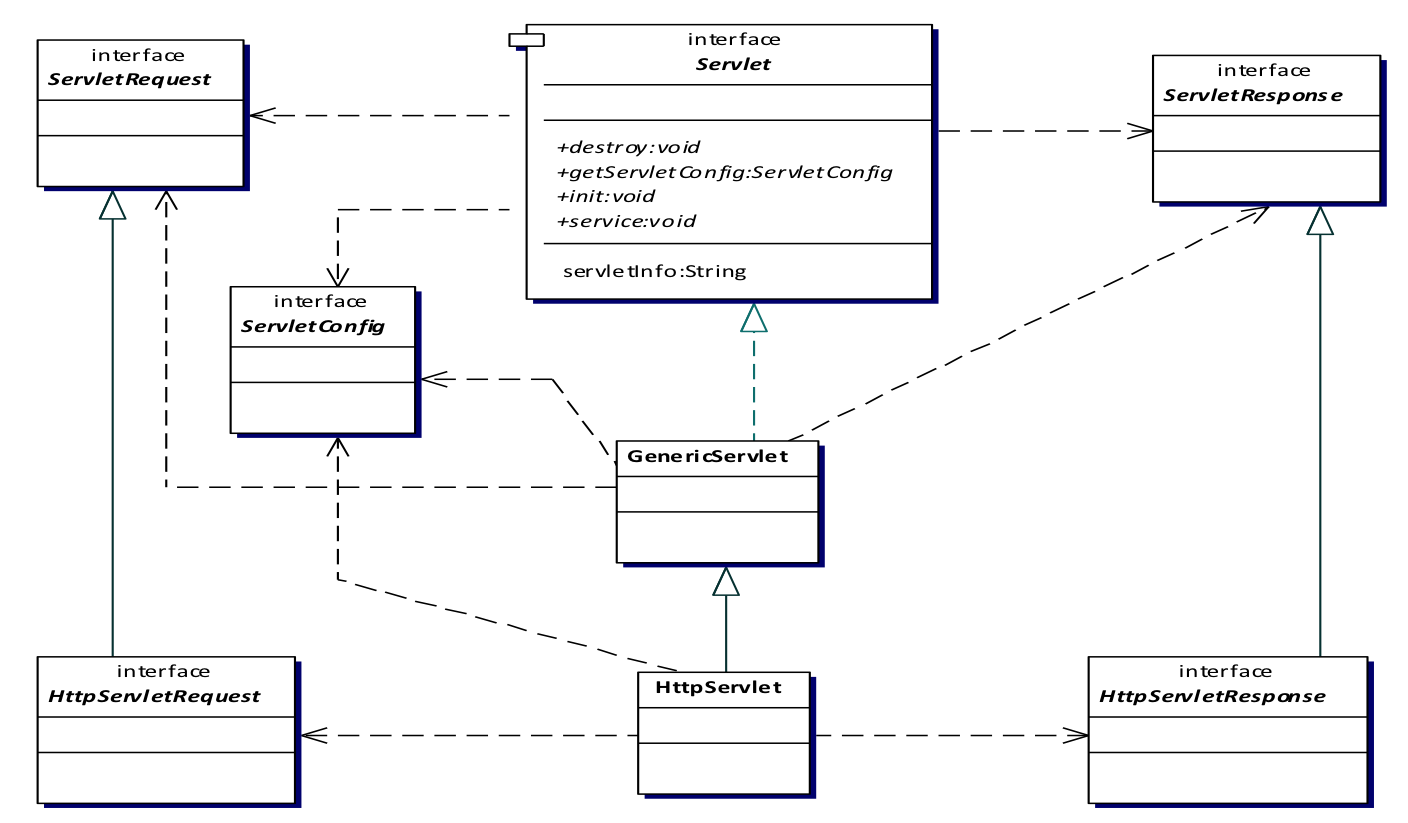
\includegraphics[width=0.85\textwidth]{fig03_02.png}
\end{figure}
\end{frame}

\section{Servlet编程}

\begin{frame}[fragile] % [fragile]参数使得能够插入代码
\frametitle{引入包} 
\begin{javaCode}
import java.io.*;
import javax.servlet.*;
import javax.servlet.http.*;
\end{javaCode}
\end{frame}

\begin{frame}[fragile] % [fragile]参数使得能够插入代码
\frametitle{类定义} 

编写接收HTTP请求并进行HTTP响应的Servlet需要继承javax.servlet.http.HttpServlet。

\begin{javaCode}
public class LoginAction extends HttpServlet {
  // Code goes on.
}
\end{javaCode}
\end{frame}

\begin{frame}[fragile] % [fragile]参数使得能够插入代码
\frametitle{重写doGet方法} 

父类HttpServlet的doGet方法是空的,没有实现任何代码,子类需要重写此方法。

\begin{javaCode}

public void doGet(HttpServletRequest request, HttpServletResponse response) 
throws ServletException, IOException {
  // Rewrite the method.
}
\end{javaCode}

当HTTP请求为GET时自动运行,每次请求都运行一次。
\end{frame}

\begin{frame}[fragile] % [fragile]参数使得能够插入代码
\frametitle{重写doPost方法} 

编写Servlet需要重写父类的doPost方法。

\begin{javaCode}
public void doPost(HttpServletRequest request, HttpServletResponse response)  
throws ServletException, IOException {
  // Rewrite the method.
}
\end{javaCode}
当请求方式为POST时自动运行,每次请求都运行一次。

{\hei\Red doGet和doPost方法都接收Web容器自动创建的请求对象和响应对象,使得Servlet能够解析请求数据和发送响应给客户端。}
\end{frame}

\begin{frame}[fragile] % [fragile]参数使得能够插入代码
\frametitle{重写init方法} 

当Web服务器创建Servlet对象后,会自动调用init方法完成初始化功能,一般将耗时的连接数据库和打开外部资源文件的操作放在init方法中。

init方法在Web容器创建Servlet对象后立即执行,且只执行一次。

\begin{javaCode}
public void init(ServletConfig config) throws ServletException {
  super.init(config);
  // 这里放置初始化工作代码.
}
\end{javaCode}

\kai 在init方法中使用Web容器传递的config对象取得Servlet的各种配置初始参数,进而使用这些参数完成读取数据库或其他外部资源。
\end{frame}

\begin{frame}[fragile] % [fragile]参数使得能够插入代码
\frametitle{重写destroy方法} 

当Web容器需要销毁Servlet对象时,一般是Web容器停止运行或Servlet源代码修改而重新部署时,Web容器自动运行destroy方法完成清理工作,如关闭数据库连接和I/O流。

\begin{javaCode}
public  void destroy() {
  try {
    cn.close();
  } catch (Exception e) {
    application.Log("登录处理关闭数据库错误" + e.getMessage());
  }
}
\end{javaCode}

\kai 代码中application为Web应用的上下文环境对象。
\end{frame}

\section{Servlet生命周期}

\begin{frame}[fragile] % [fragile]参数使得能够插入代码
\frametitle{Servlet的运行过程} 
\begin{enumerate}\kai
\item 用户在浏览器请求ServletURL地址。
\item Web容器接收到请求,检查是Servlet请求,将处理交给Servlet引擎。
\item Servlet引擎根据URL地址检查是否有Servlet映射,如果没有则返回错误信息给浏览器。
\item 有servlet映射时,先检查是否有实例在运行。
\item 如果没有实例运行,则创建Servlet类的对象,调用其构造方法,然后调用init()方法。
\item 如果有实例在运行,则根据请求的方法是GET或POST,自动调doGet()或doPost()方法。将请求对象和响应对象传给doGet()或doPost()方法。
\item 在doGet()或doPost()方法内通过HttpServletRequest的请求对象分析出用户发送的请求信息。
\item 按用户的要求进行业务处理。
\item 通过HttpServletResponse响应对象向浏览器发送响应信息。
\end{enumerate}
\end{frame}

\begin{frame}[fragile] % [fragile]参数使得能够插入代码
\frametitle{Servlet处理流程} 
\begin{figure}
\centering
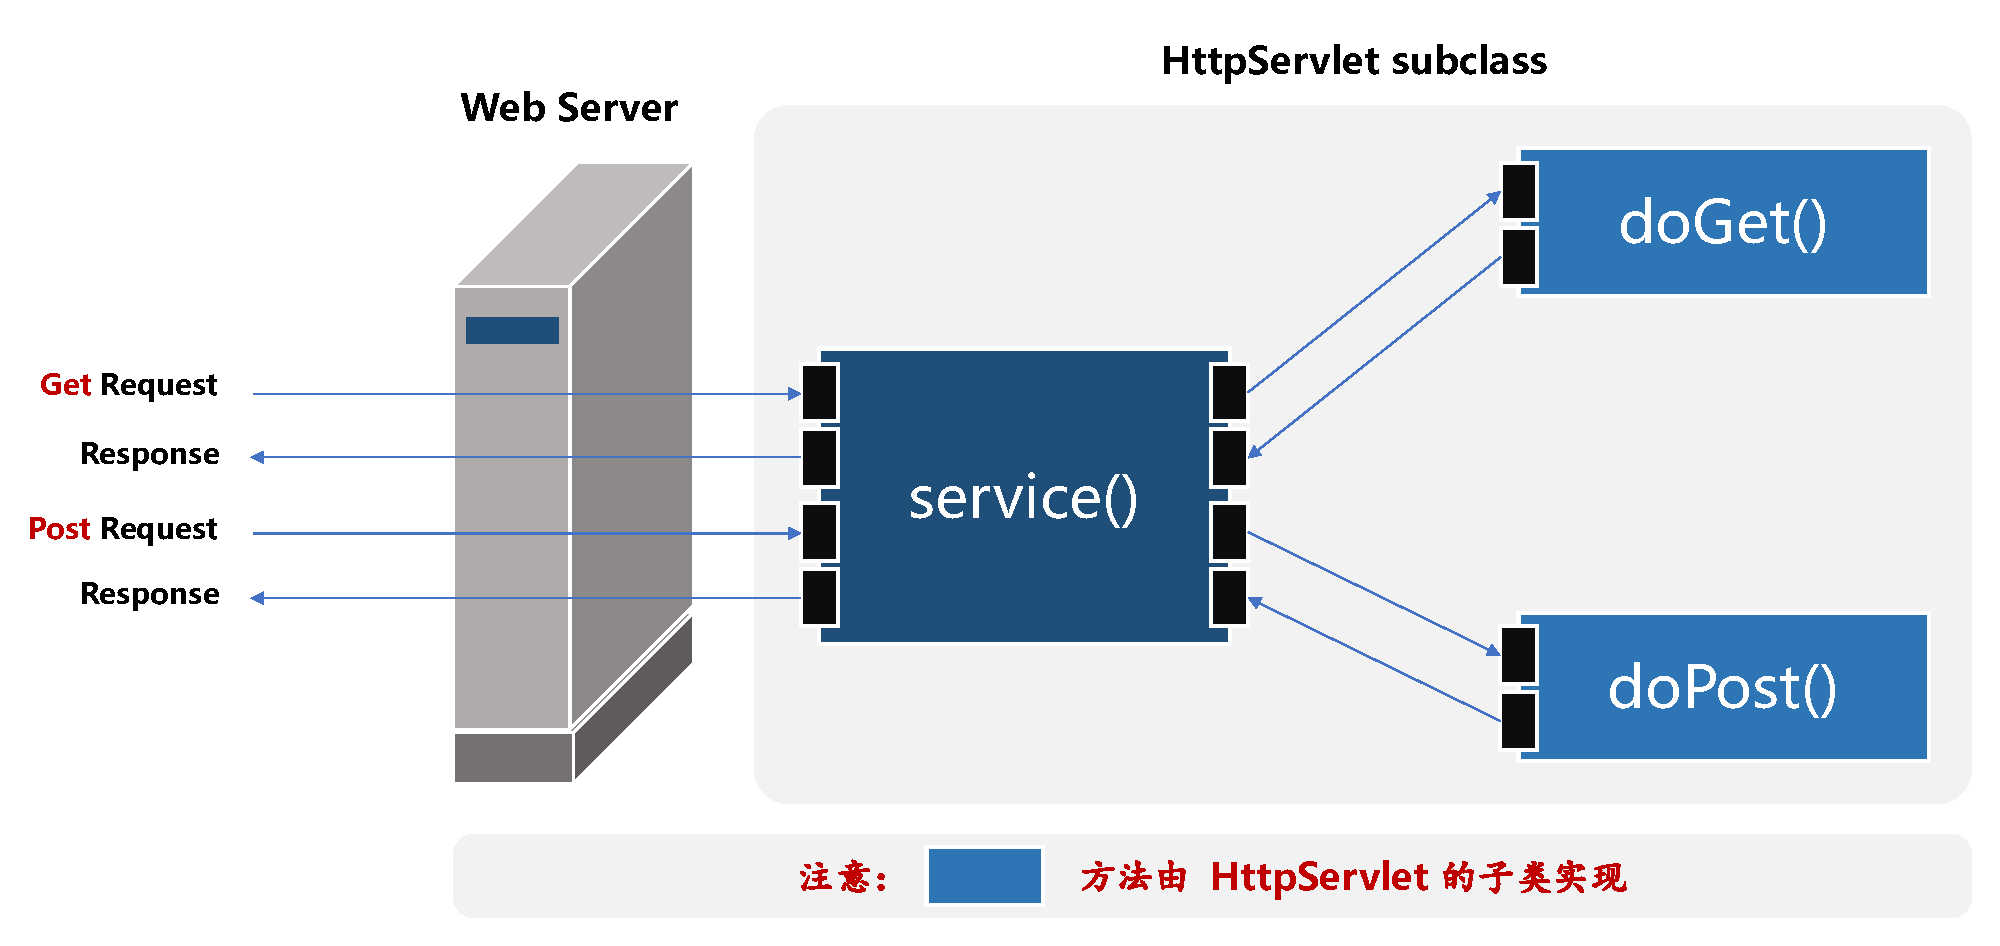
\includegraphics[width=\textwidth]{fig-servlet-mechanism.pdf}
\end{figure}
\end{frame}

\section{Servlet配置}

\begin{frame}[fragile] % [fragile]参数使得能够插入代码
\frametitle{Servlet配置}
\begin{itemize}
\item Servlet作为Web组件可以处理HTTP请求/响应,因此对外要求一个唯一的URL地址。
\item Servlet是一个Java类文件,不像JSP那样直接存放在Web目录下就能获得URL请求访问地址。
\item Servlet必须在Web的配置文件{\Red /WEB-INF/web.xml}中进行配置和映射才能响应HTTP请求。
\item Servlet的配置分为{\hei 声明和映射}两个步骤。
\end{itemize}
\end{frame}

\begin{frame}[fragile] % [fragile]参数使得能够插入代码
\frametitle{Servlet配置}
\wxd{Servlet声明}

通知Web容器Servlet的存在。

\begin{xmlCode}
<servlet>
  <servlet-name>loginaction</servlet-name>
  <servlet-class>com.city.oa.action.LoginAction</servlet-class>
</servlet>  
\end{xmlCode}

<servlet-name> 声明Servlet的名字,要求在一个web.xml文件内名字唯一。\\
<servlet-class> 指定Servlet的全名,即包名.类名。\\
\end{frame}

\begin{frame}[fragile] % [fragile]参数使得能够插入代码
\frametitle{Servlet配置}
\ttc{Servlet初始参数}

在Servlet的声明中可以配置Servlet初始参数,如数据库的Driver、URL、账号和密码等信息。在Servlet中可以读取这些信息,避免在Servlet代码中定义这些信息,修改时无需重新编译Servlet。

\begin{xmlCode}
<servlet>
  <init-param>
    <param-name>driver</param-name>
    <param-value>sun.jdbc.odbc.JdbcOdbcDriver</param-value>
  </init-param>
</servlet>
\end{xmlCode}

在Servlet中取得以上定义的参数的方法:

\begin{javaCode}
String driver = config.getInitParameter("driver");
\end{javaCode}
\end{frame}

\begin{frame}[fragile] % [fragile]参数使得能够插入代码
\frametitle{Servlet配置}
\ttc{Servlet启动时机}

在配置Servlet时,可以指示Servlet跟随Web容器一起自动启动。这时,Servlet就可以在没有请求的情形下,进行实例化和初始化,完成特定任务。自启动Servlet的配置语法:

\begin{xmlCode}
<load-on-startup>2</load-on-startup>
\end{xmlCode}

数字越小越先启动,0表示紧跟Web容器启动后第一个启动。
\end{frame}

\begin{frame}[fragile] % [fragile]参数使得能够插入代码
\frametitle{Servlet配置}
\wxd{Servlet映射}
\begin{itemize}
\item 任何Web文档在Internet上都要有一个URL地址才能被请求访问。
\item Servlet不能像JSP一样直接放在Web的发布目录上,需要单独映射URL地址。
\item 在{\Red /WEB-INF/web.xml}中进行Servlet的URL映射。
\end{itemize}

\ttc{映射语法}

\begin{xmlCode}
<servlet-mapping>
  <servlet-name>servlet name</servlet-name>
  <url-pattern>URL</url-pattern>
</servlet-mapping>
\end{xmlCode}
{\kai 其中,servlet name与Servlet声明中的名称要一致。}
\end{frame}

\begin{frame}[fragile] % [fragile]参数使得能够插入代码
\frametitle{Servlet配置}
\wxd{Servlet映射}

\ttc{映射地址方式 \ding{182} 绝对地址方式映射}
\begin{xmlCode}
<servlet-mapping>
  <servlet-name>LoginAction</servlet-name>
  <url-pattern>/login.action</url-pattern>
</servlet-mapping>
\end{xmlCode}
\end{frame}

\begin{frame}[fragile] % [fragile]参数使得能够插入代码
\frametitle{Servlet配置}
\wxd{Servlet映射}

\ttc{映射地址方式 \ding{183} 匹配目录模式映射方式}
\begin{xmlCode}
<servlet-mapping>
  <servlet-name>MainAction</servlet-name>
  <url-pattern>/main/*</url-pattern>
</servlet-mapping>
\end{xmlCode}

在这个配置中,只要以/main开头的任何URL都能请求此Servlet。
\end{frame}

\begin{frame}[fragile] % [fragile]参数使得能够插入代码
\frametitle{Servlet配置}
\wxd{Servlet映射}

\ttc{映射地址方式 \ding{184} 匹配扩展名模式映射方式}
\begin{xmlCode}
<servlet-mapping>
  <servlet-name>MainAction</servlet-name>
  <url-pattern>*.action</url-pattern>
</servlet-mapping>
\end{xmlCode}

以上配置中扩展名为action的任何请求均被此Servlet响应。

{\Red\kai 注意:不能混合使用以上两种配置模式,否则会在Web项目部署并运行时产生运行时错误。}

如以下配置是错误的:

\begin{xmlCode}
<servlet-mapping>
  <servlet-name>MainAction</servlet-name>
  <url-pattern>/main/*.action</url-pattern>
</servlet-mapping>
\end{xmlCode}
\end{frame}

\section{Servlet部署}

\begin{frame}[fragile] % [fragile]参数使得能够插入代码
\frametitle{Servlet部署}

编译好的Servlet class文件应该放到指定的Web应用目录下,才能被Web容器找到,这个目录为:\\
{\Red /WEB-INF/classes/package/FileName.class}

例如Servlet类LoginAction:
\begin{javaCode}
package city.oa.servlet;
public class LoginAction extends HttpServlet {
  //     
}
\end{javaCode}

存放目录为:
{\Blue /WEB-INF/classes/city/oa/servlet/LoginAction.class}
\end{frame}

\section{Servlet示例} 

\begin{frame}[fragile] % [fragile]参数使得能够插入代码
\frametitle{Servlet示例} 
\ttc{Eclipse}

New Project \ding{223} Web \ding{223} Dynamic Web Project \ding{223} Next >

---------------------------------------------------------------------------\\
Project name: {\Blue sample.servlet}\\
Target runtime\\ {\Blue Apache Tomcat v8.0}\\
Dynamic web module version\\ 3.0\\
Configuration\\ {\Blue Default Configuration for Apache Tomcat v8.0}\\
---------------------------------------------------------------------------\\
\ding{223} Next >
\end{frame}

\begin{frame}[fragile] % [fragile]参数使得能够插入代码
\frametitle{Servlet示例} 

---------------------------------------------------------------------------\\
Source folder on build path: \\ {\Blue src}\\
%%Default output folder: \\ {\Blue WebContent/WEB-INF/classes}\\
---------------------------------------------------------------------------\\

\ding{223} Next >

---------------------------------------------------------------------------\\
{\Blue\ding{52}} Generate web.xml deployment descriptor\\
---------------------------------------------------------------------------\\
\ding{223} Finish
\end{frame}

\begin{frame}[fragile] % [fragile]参数使得能够插入代码
\frametitle{Servlet示例} 

\ttc{WebContent/WEB-INF/web.xml}

Add following statements between <web-app> and </web-app>.

\begin{xmlCode}
  <servlet>
    <servlet-name>HelloServlet</servlet-name>
    <servlet-class>ouc.javaweb.HelloServlet</servlet-class>
    <load-on-startup>0</load-on-startup>
  </servlet>
    
  <servlet-mapping>
    <servlet-name>HelloServlet</servlet-name>
    <url-pattern>/hello</url-pattern>
  </servlet-mapping>  
\end{xmlCode}
\end{frame}

\begin{frame}[fragile] % [fragile]参数使得能够插入代码
\frametitle{Servlet示例} 

\ttc{Java Resources/src}

Create java class file named ``HelloServlet.java''.

\begin{javaCode}
package ouc.javaweb;

import java.io.IOException;
import java.io.PrintWriter;
import javax.servlet.ServletException;
import javax.servlet.http.HttpServlet;
import javax.servlet.http.HttpServletRequest;
import javax.servlet.http.HttpServletResponse;

public class HelloServlet extends HttpServlet {
  public void doGet(HttpServletRequest request, HttpServletResponse response)
  throws ServletException, IOException {
    response.setContentType("text/html");
    response.setCharacterEncoding("UTF-8");
    PrintWriter out = response.getWriter();
    out.println("<html>");
    out.println("<head><title>A Servlet Sample</title></head>");
    out.println("<body>");
    out.println("<h1>Hello, Servlet!</h1>");
    out.println("A Servlet is a Java-based server-side web technology. ");
    out.println("</body></html>"););
    out.flush();
    out.close();
  }
}
\end{javaCode}
\end{frame}

\begin{frame}[fragile] % [fragile]参数使得能够插入代码
\frametitle{Servlet示例} 

sample.servlet \ding{223} 鼠标右键 \ding{223} Run as \ding{223} Run on Server

 \ding{223} Choose an existing server \ding{223} Tomcat v8.0 Server at localhost \ding{223} Finish

在浏览器中请求页面{\Blue http://localhost:8080/sample.servlet/hello}。

\end{frame}


\begin{frame}
  \frametitle{本节习题}

  \tta{问答题}
  
  \begin{enumerate}
  \item Servlet和一般Java类的区别是什么?
  \item 简述Servlet的生命周期。
  \item 简述Servlet与URL地址的映射方式(包括web.xml配置和基于注解)。
  \end{enumerate}

  \tta{小编程}
  
  \begin{enumerate}
  \item 编写一个能够计数访问次数的Servlet,每次请求次数增加1,并显示当前总访问次数。
  \end{enumerate}
\end{frame}
% TKS %%%%%%%%%%%%%%%%%%%%%%%%%%%%%%%%%%%%%%%%%%%%%%
\begin{frame}
\centering
{\Huge \textcolor{blue}{THE END}} \\
\vspace{5mm}
{\Large wangxiaodong@ouc.edu.cn} \\
\end{frame}
%%%%%%%%%%%%%%%%%%%%%%%%%%%%%%%%%%%%%%%%%%%%%%%%%%
\end{document}
